\documentclass{article}
\usepackage[utf8]{inputenc}
\usepackage{graphicx}
\usepackage{amsmath}
\usepackage{titling}
\usepackage{pdflscape}

\setlength{\droptitle}{-10em}
\pagestyle{empty}

\title{Lab. 1 - Resilienza di una rete di comunicazione}
\author{Ballarin Simone, Gobbo Alessio, Rossi Daniel}
\date{March 2019}

\begin{document}
\maketitle

\section*{Domanda 1}
Il grafo reale, che appartiene alla famiglia dei grafi non orientati, è formato da un numero di nodi pari a 6474 collegati tra loro da 12572 archi, non considerando eventuali cappi (arco con uguali estremi).\\
Ci viene richiesto di generare grafi non orientati casuali con medisime caratteristiche di cardinalità del grafo reale utilizzando gli algoritmi ER e UPA.\\
A tal fine si è reso necessario calcolare la probabilità \textit{p} per l'algoritmo ER, mentre per quanto riguarda il parametro \textit{m} dell'algoritmo UPA ci è stato fornito nella consegna.
\subsection*{Calcolo probabilità \textit{p}}
Dato il grafo $ER(V,E)$ da generare esso dovrà avere le seguenti caratteristiche:
\begin{itemize}
	\item $|V|= 6474$
	\item $|E| \approx 12572$
\end{itemize}
Sia $X$ una variabile aleatoria binomiale $X=Bin(\frac{|V|(|V|-1)}{2},p)$:
\begin{itemize}
	\item $\frac{|V|(|V|-1)}{2}$: numero massimo di possibili archi creabili;
	\item $p$ : probabilità che venga creato un arco.
\end{itemize} 
Questa varibile descrive il numero di successi (archi creati) nella generazione del grafo $ER(V,E)$.\\
Vengono effettuate $\frac{|V|(|V|-1)}{2}$ scelte, ciascuna delle quali corrisponde alla possibile creazione di un arco tra due nodi non identici con probabilità \textit{p} ignota.\\
Volendo avere mediamente un numero di archi $|E| \approx 12572$, questo porta ad aspettarci che il valore atteso $E(X) = 12572$.\\
Sappiamo inoltre che il valore atteso di una variabile aleatoria binomiale può essere espresso come  $E(X)=\frac{|V|(|V|-1)}{2}p$.\\
Possiamo ora impostare il seguente sistema:
$$
\begin{cases}
	E(X) = 12572               \\ 
	E(X)=\frac{|V|(|V|-1)}{2}p 
\end{cases}
$$
Da cui otteniamo la probabilità $p = 2\frac{12572}{|V|(|V|-1)} = 0.000600006652953 \approx 0.0006$
\begin{landscape}
	\begin{figure}
		\centering
		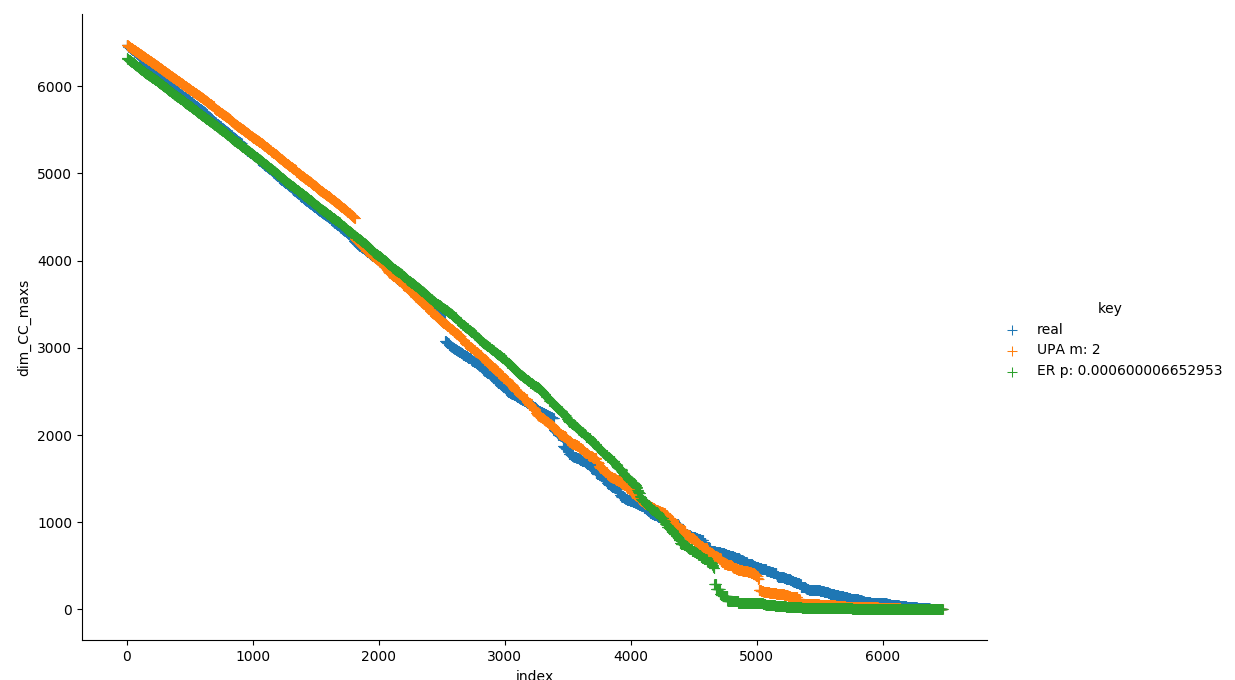
\includegraphics[width=1.8\textwidth]{../grafici/Figure_4}
		\caption{Grafico resilienza attacco casuale.}
	\end{figure}
\end{landscape}

\newpage
\section*{Domanda 2}
Al fine di valutare il comportamento dei tre grafi colpiti da un attacco casuale, abbiamo inserito nel grafico precedente due rette:
\begin{itemize}
	\item retta orizzontale corrispondete al limite di resilienza del 75\% (4576 nodi);
	\item retta verticale indica il superamento del 20\% (1295 nodi) dei nodi rimossi. 
\end{itemize}
Come si può osservare, dopo la rimozione del 20\% dei nodi, tutti e tre i gruppi di punti sono oltre il limite di resilienza fissato al 75\%, ottenendo valori di resilienza simili.\\
Dato che la natura dell'attacco è casuale la riesecuzione dello stesso porterebbe ad ottenere risultati leggermente diversi, osservando però i gruppi di punti globalmente possiamo constatare una forte similarità in termini di linearità della diminuzione della resilienza.\\
In conclusione possiamo dire che i gruppi di punti sono essenzialmente comparabili, l'unica differenza riscontrabile si può apprezzare nella parte finale dell'asse orrizzontale in cui le varie resilienze si discostano significativamente.

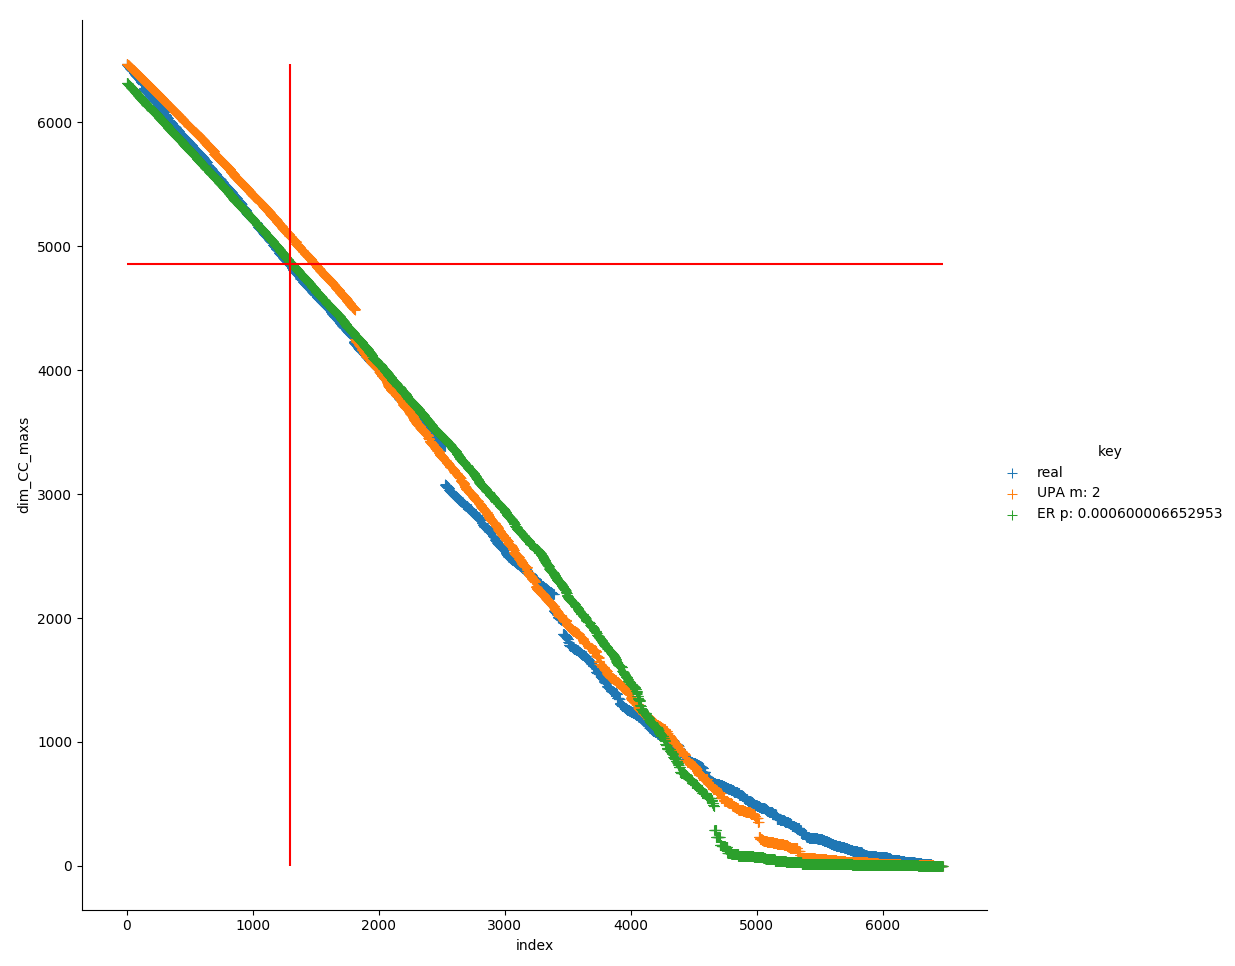
\includegraphics[width=1.0\textwidth]{../grafici/Figure_2}

\newpage
\begin{landscape}
    \section*{Domanda 3}
Abbiamo effettuato l'attacco con strategia max-degree. Il seguente grafico presenta la correlazione tra nodi rimossi e dimensione della componente connessa massima come richiesto dalla domanda.
	\begin{figure}[h]
		\centering
		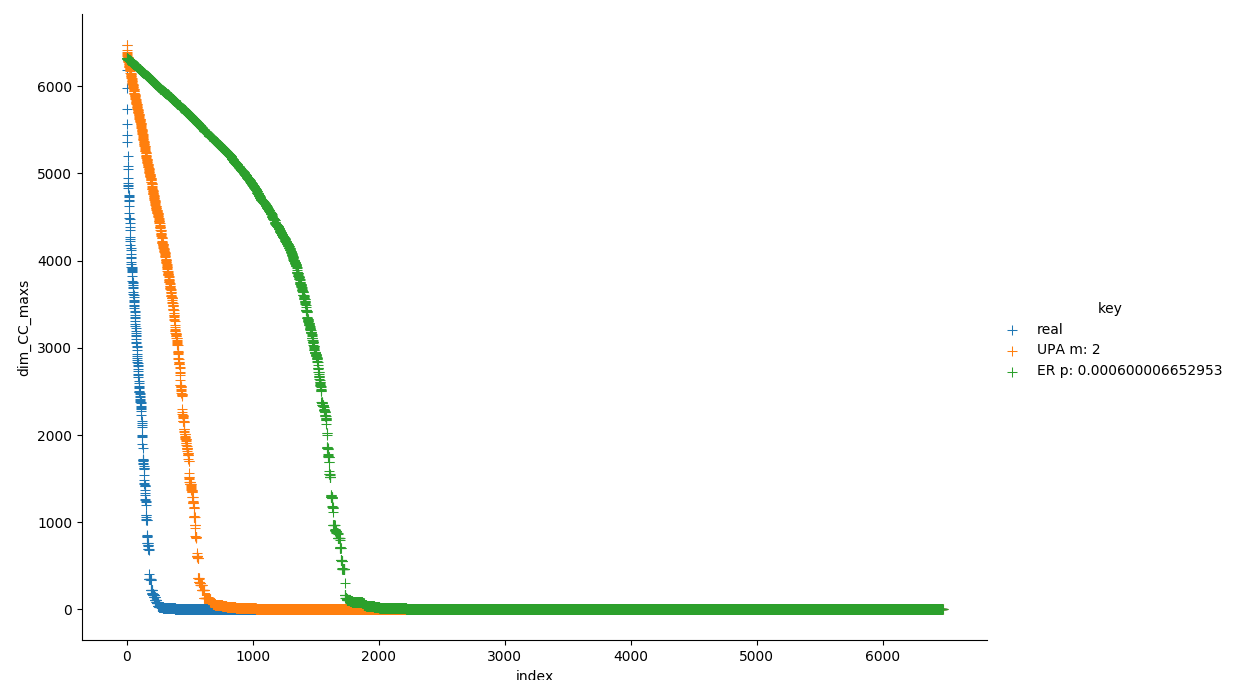
\includegraphics[width=1.25\textwidth]{../grafici/Figure_3}
		\caption{Grafico resilienza attacco max-degree.}
	\end{figure}
\end{landscape}

\section*{Domanda 4}
In maniera analoga a quanto fatto precedentemente, si sono inserite due rette:
\begin{itemize}
	\item retta orizzontale corrispondete al limite di resilienza del 75\% (4576 nodi);
	\item retta verticale indica il superamento del 20\% (1295 nodi) dei nodi rimossi. 
\end{itemize}
In questo caso tutti i grafi sono sotto la soglia di resilienza presentando però andamenti estremamente differenti.\\
Il grafo reale è quello che presenta il comportamento peggiore, in quanto presenta una caduta repentina immediatamente dopo le prime rimozioni e dopo circa 200 rimozioni ha relienza quasi nulla.\\
Il grafo UPA invece ha una caduta meno rapida comparata al grafo reale, ma comunque veloce infatti la resilienza si annulla quasi completamente già dopo 700 rimozioni.
Il grafo ER risulta invece quello più resistente: nonostante non riesca a mantenersi sopra la soglia dopo il 20\% delle rimozioni è quello che si avvicina maggiormente. Fino a quasi 1000 rimozioni ha una decrescita quasi lineare, mentra tra 1000 e 1200 rimozioni il tasso di decrescita aumenta fino a diventare esponenziale dopo aver superato il limite delle 1200 rimozioni.\\
Queste differenze le imputiamo alle diverse topologie che i tre grafi presentano, infatti dato che la scelta non è più casuale, queste influenzano gli effetti dell'attacco.\\
ER avendo una varianza del grado più bassa rispetto agli altri è quello che si comporta meglio.\\
UPA invece per come lavora l'algoritmo tende a creare pochi nodi con grado alto e tanti nodi con grado basso che si collegano a questi.\\
L'attacco intelligente, rimuovendo i pochi nodi a grado alto, ottiene dei buoni risultati nell'abbassamento della resilienza.\\
Il grafo reale, invece, intuiamo essere caratterizzato da un basso numero di nodi ad alto grado (le città più importanti) ai quali sono collegati un certo numero di nodi a basso grado non condivisi (le periferie delle città). A differenza di UPA questi nodi di grado alto non sono collegati a meno nodi (per motivi geografici) e quindi per questa ragione presenta una robustezza inferiore.

Al fine di avere una maggiore comprensione della topologia abbiamo deciso di realizzare tre rappresentazioni grafiche dei vari grafi. Si rappresentano i nodi con cerchi di raggio proporzionale al grado.

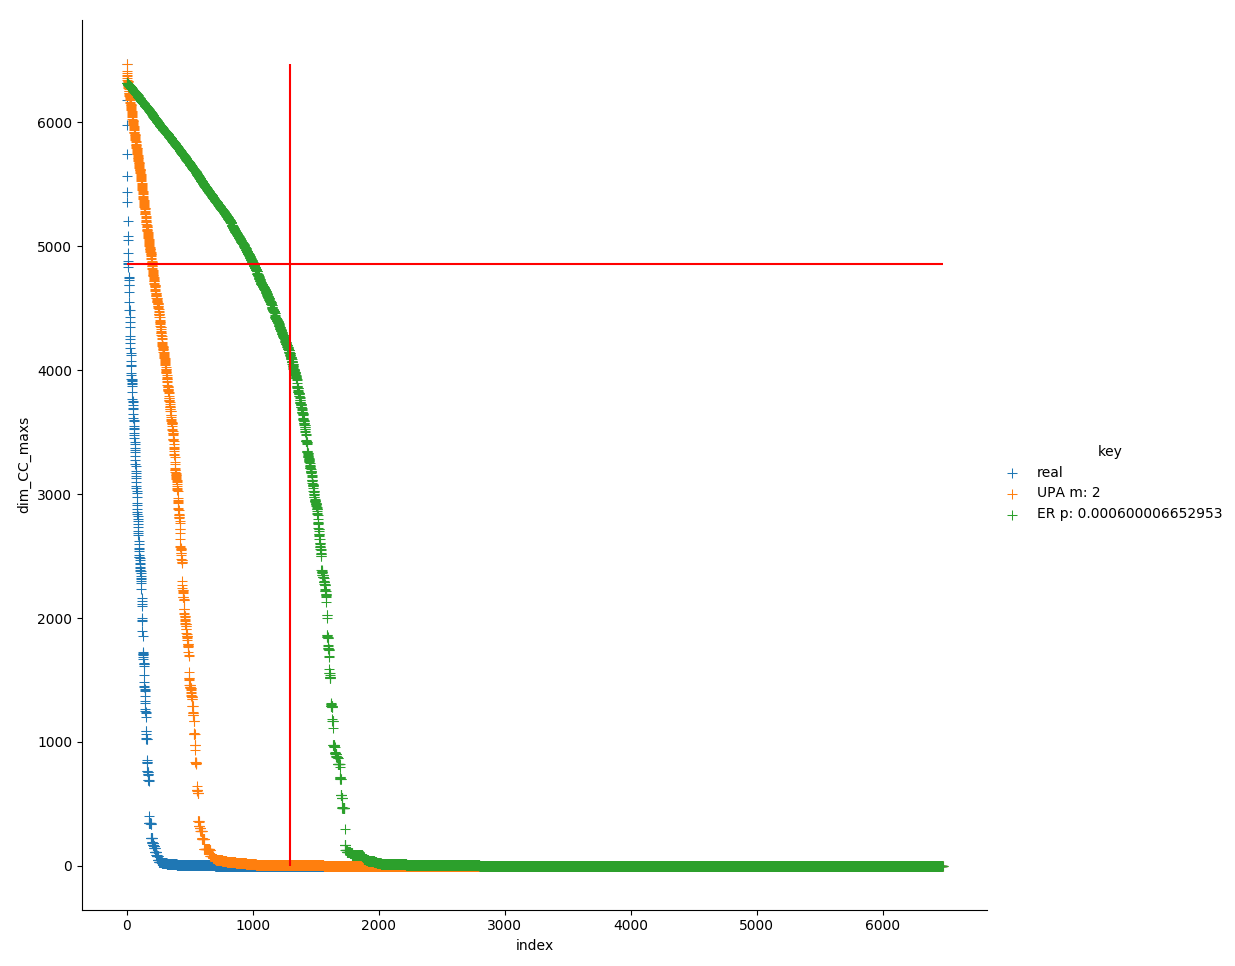
\includegraphics[width=0.9\textwidth]{../grafici/Figure_1}

\section*{Domanda 5}
In allegato alla consegna sono stati inseriti i codice sorgente Python.
    
\end{document}
